\documentclass{beamer}
\usepackage[utf8]{inputenc}
\usepackage[english]{babel}
\usepackage{ragged2e}
\usepackage{graphicx}
\usepackage{amsmath}
\usepackage{array}
\usepackage{url}
\usepackage{tikz}
\usetikzlibrary{positioning}
\usetheme{Madrid}
\usecolortheme{beaver}
\useinnertheme{rectangles}
\setbeamercolor{footline}{fg=white,bg=black}
\setbeamertemplate{bibliography item}{\insertbiblabel}
\beamertemplatenavigationsymbolsempty

\title[Placement Hub]{Placement Hub \\ A Web-Based Campus Placement Management System}
\author[Group 18]{
\Large Group No: 18\\\\
\large
Fathima Safeeda K \hspace{1cm} (KKE23CSD024)\\
Fimsha Palakkal \hspace{1.2cm} (KKE23CSD025)\\
Hima P H \hspace{1.8cm} (KKE23CSD030)\\
Sreehari S \hspace{1.6cm} (KKE23CSD062)
}
\institute[GEC Kozhikode]{
\large
S\textsubscript{6} B.Tech Computer Science \& Design\\
Government Engineering College, Kozhikode\\[6pt]
Guided By: \textbf{Ms. Shimna M S}\\
Assistant Professor, Dept. of CSE
}
\date{March 2026}

\newcommand{\imgplaceholder}[2]{
  \begin{center}
  \fbox{
    \begin{minipage}[c][0.42\textheight][c]{0.82\textwidth}
      \centering
      \textbf{#1}\\[4pt]
      Place the image file here before final compilation.\\
      Expected file: \texttt{#2}
    \end{minipage}
  }
  \end{center}
}

\newcommand{\safeimage}[3]{
  \IfFileExists{#2}{
    \begin{center}
    \includegraphics[#1]{#2}
    \end{center}
  }{
    \imgplaceholder{#3}{#2}
  }
}

\begin{document}

\frame[plain]{\titlepage}

\begin{frame}[plain]{Overview}
\tableofcontents
\end{frame}

\section{Introduction}
\begin{frame}{Introduction}
\justifying
Campus placement activity involves collecting student data, managing company details,
publishing opportunities, validating eligibility, handling resumes, tracking applications,
and communicating results. In many colleges these tasks are still performed through
spreadsheets, emails, and isolated portals, which creates delay, duplication, and low
visibility for all stakeholders.

\vspace{6pt}
\textbf{Placement Hub} is developed as a centralized web platform for students, companies,
and the placement cell to streamline the complete recruitment workflow from registration
to selection tracking.
\end{frame}

\section{Motivation}
\begin{frame}{Motivation}
\justifying
\textbf{Societal need}
\begin{itemize}
\item Reduce confusion and missed opportunities for students during placement drives
\item Improve transparency between students, recruiters, and placement officers
\item Create a structured digital record of campus recruitment activity
\end{itemize}

\textbf{Technical need}
\begin{itemize}
\item Replace manual verification and repeated data entry
\item Enforce eligibility, access control, and role-based workflows
\item Support faster communication, status updates, and placement analytics
\end{itemize}
\end{frame}

\section{Objective}
\begin{frame}{Objective}
\begin{itemize}
\item Automate the end-to-end campus placement process
\item Provide separate dashboards for student, company, and admin roles
\item Support secure resume upload, verification, and controlled visibility
\item Improve application tracking, communication, and recruitment efficiency
\item Maintain placement statistics and operational monitoring in one system
\end{itemize}
\end{frame}

\section{Related Works}
\begin{frame}{Literature Survey / Related Works}
\scriptsize
\renewcommand{\arraystretch}{1.15}
\begin{center}
\begin{tabular}{|p{2.5cm}|p{2.9cm}|p{2.6cm}|p{2.7cm}|}
\hline
\textbf{System} & \textbf{Focus} & \textbf{Merits} & \textbf{Demerits} \\ \hline
Campus Recruitment Automation System & Job application and shortlisting flow & Automates form submission and candidate filtering & Limited admin analytics and weak security controls \\ \hline
Online Campus Placement System & Recruiter vacancy publishing and student application & Easy access to openings and application tracking & Often lacks detailed verification and reporting modules \\ \hline
University Placement Management System & Central storage of placement records and schedules & Better data organization and coordination & Usually no real-time status updates or feedback support \\ \hline
Student Job Placement Portal & Profile creation and job search support & Simplifies resume-based job application & Limited communication channel between HR and placement cell \\ \hline
\textbf{Placement Hub} & Unified placement workflow with verification, dashboards, and role-based control & Centralized platform, status tracking, verification, feedback, and analytics & Can be extended further with interview scheduling and bulk automation \\ \hline
\end{tabular}
\end{center}
\end{frame}

\section{Problem Statement}
\begin{frame}{Problem Statement}
\justifying
Design and develop a secure web-based placement management system that automates
student registration, company onboarding, job posting, application tracking,
resume verification, and administrative monitoring in order to improve efficiency,
transparency, data consistency, and communication during campus recruitment.
\end{frame}

\section{Functional Requirements}
\begin{frame}{Functional Requirements}
\begin{itemize}
\item Student registration, login, profile editing, and scorecard upload
\item College email restriction and secure role-based authentication
\item Company registration, profile management, and job posting
\item Student job application with eligibility and status tracking
\item Resume upload, public/private visibility control, and verification workflow
\item Applicant review, shortlisting, rejection, and mail support
\item Admin dashboard with company management, resume review, feedback review, and placement statistics
\end{itemize}
\end{frame}

\section{Module Description}
\begin{frame}{Module Description}
\scriptsize
\renewcommand{\arraystretch}{1.12}
\begin{center}
\begin{tabular}{|p{2.15cm}|p{2.2cm}|p{3.85cm}|p{2.15cm}|}
\hline
\textbf{Module} & \textbf{Input} & \textbf{Processing} & \textbf{Output} \\ \hline
Student Module & Personal details, college email, CGPA, scorecard, resume, applications & Authentication, access validation, profile update, resume upload, visibility control, application submission, status tracking, feedback submission & Updated profile, verified/private/public resume state, application status \\ \hline
Company Module & Company details, HR details, job description, eligibility criteria & Company authentication, company profile update, job creation/edit/delete, applicant review, shortlist/reject action, resume viewing & Job listings, shortlisted/rejected applicants, updated company data \\ \hline
Admin Module & Student/company records, resumes, feedback, placement count & Admin login, company onboarding, credential generation, resume verification/rejection, dashboard monitoring, profile and team management & Approved records, analytics, verified resumes, system oversight \\ \hline
\end{tabular}
\end{center}
\end{frame}

\section{System Architecture}
\begin{frame}{System Architecture}
\safeimage{width=0.92\linewidth}{sys_arch.png}{System Architecture Diagram}
\end{frame}

\section{Detailed Design}
\begin{frame}{Level 2 DFD / Data Flow}
\footnotesize
\begin{center}
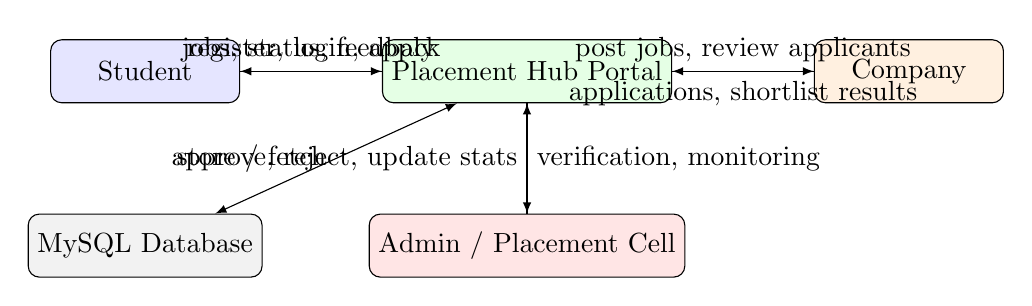
\begin{tikzpicture}[node distance=1.3cm,>=latex]
\node[draw,rounded corners,fill=blue!10,minimum width=2.4cm,minimum height=0.8cm] (student) {Student};
\node[draw,rounded corners,fill=green!10,right=1.8cm of student,minimum width=3.2cm,minimum height=0.8cm] (portal) {Placement Hub Portal};
\node[draw,rounded corners,fill=orange!12,right=1.8cm of portal,minimum width=2.4cm,minimum height=0.8cm] (company) {Company};
\node[draw,rounded corners,fill=red!10,below=1.4cm of portal,minimum width=2.7cm,minimum height=0.8cm] (admin) {Admin / Placement Cell};
\node[draw,rounded corners,fill=gray!10,below=1.4cm of student,minimum width=2.6cm,minimum height=0.8cm] (db) {MySQL Database};

\draw[->] (student) -- node[above]{register, login, apply} (portal);
\draw[->] (portal) -- node[above]{jobs, status, feedback} (student);
\draw[->] (company) -- node[above]{post jobs, review applicants} (portal);
\draw[->] (portal) -- node[right]{verification, monitoring} (admin);
\draw[->] (admin) -- node[left]{approve, reject, update stats} (portal);
\draw[<->] (portal) -- node[left]{store / fetch} (db);
\draw[->] (portal) -- node[below]{applications, shortlist results} (company);
\end{tikzpicture}
\end{center}

\vspace{4pt}
\justifying
The level 2 flow shows how user data, job data, resume data, and application status move
between the three actors and the centralized database through the Placement Hub portal.
\end{frame}

\section{Implementation Details}
\begin{frame}{Implementation Details}
\small
\textbf{Software tools and languages}
\begin{itemize}
\item Frontend: HTML, CSS, JavaScript
\item Backend: PHP with mysqli
\item Database: MySQL / MariaDB
\item Version Control: Git and GitHub
\item Development Environment: XAMPP, VS Code
\end{itemize}

\textbf{Libraries / platform support}
\begin{itemize}
\item Session management and password hashing in PHP
\item Prepared statements for database operations
\item Progressive Web App support through manifest and service worker
\item SMTP/mail fallback utility for email handling
\end{itemize}
\end{frame}

\begin{frame}{Implementation Highlights}
\small
\begin{itemize}
\item Student access can be restricted to official college email domains
\item Email verification flow is supported for student account activation
\item Student lifecycle control can expire access after graduation period
\item Resume files support PDF, DOC, and DOCX with role-based access rules
\item Companies can view applicant profile, resume, and KTU scorecard
\item Admin can verify or reject public resumes and monitor placement statistics
\item Admin profile and placement team member details are configurable from the system
\end{itemize}
\end{frame}

\section{Version Control}
\begin{frame}{Version Control Used}
\justifying
\textbf{GitHub} was used for version control and collaboration.

\begin{itemize}
\item Source code was maintained in a central Git repository
\item Features and corrections were pushed incrementally during development
\item Remote history helped track progress, fixes, and deployment-ready versions
\item Git-based workflow reduced code loss and improved team coordination
\end{itemize}
\end{frame}

\section{Task Allocation}
\begin{frame}{Task Allocation}
\begin{itemize}
\item Fathima Safeeda K: UI design, student registration, student dashboard integration
\item Fimsha Palakkal: Company registration, company dashboard, job posting workflow
\item Hima P H: Admin dashboard, verification workflow, monitoring and control panels
\item Sreehari S: Database design, backend integration, validation and connectivity
\end{itemize}
\end{frame}

\section{Project Plan}
\begin{frame}{Overall Schedule}
\scriptsize
\renewcommand{\arraystretch}{1.12}
\begin{center}
\begin{tabular}{|p{4.25cm}|p{2.35cm}|p{2.35cm}|}
\hline
\textbf{Work} & \textbf{Planned Date} & \textbf{Completion} \\ \hline
Topic Finalization & 04-12-2025 & 08-12-2025 \\ \hline
SRS Documentation & 15-12-2025 & 15-12-2025 \\ \hline
Authentication and Login Pages & 18-12-2025 & 22-12-2025 \\ \hline
Student and Company Registration & 29-12-2025 & 08-01-2026 \\ \hline
Dashboard Frontend Development & 13-01-2026 & 09-02-2026 \\ \hline
Database Design and Table Setup & 06-02-2026 & 10-02-2026 \\ \hline
Backend Integration & 11-02-2026 & 25-02-2026 \\ \hline
Resume and Job Modules & 26-02-2026 & 05-03-2026 \\ \hline
Testing, Debugging, Final Corrections & 06-03-2026 & 20-03-2026 \\ \hline
Final Submission Preparation & 21-03-2026 & 25-03-2026 \\ \hline
\end{tabular}
\end{center}
\end{frame}

\section{Results}
\begin{frame}{Results Achieved}
\small
\begin{itemize}
\item Student, company, and admin roles are successfully implemented
\item Job posting, job application, status update, and resume workflows are working
\item Admin dashboard displays student count, company count, resume count, and placement count
\item Resume verification, feedback collection, and company management are integrated
\item Newly added features improved security, usability, and monitoring of the system
\end{itemize}
\end{frame}

\begin{frame}{Newly Added Features}
\small
\begin{itemize}
\item Student email-domain based access restriction
\item Student email verification flow and resend support structure
\item Access-expiry logic for graduated students
\item KTU scorecard upload and recruiter viewing
\item Resume public/private toggle with verification status display
\item Feedback submission and admin-side feedback review
\item Dynamic admin team-member management
\item Hosting-ready email sender with SMTP fallback
\item PWA manifest and service worker support
\end{itemize}
\end{frame}

\section{Screenshots}
\begin{frame}{Login Page}
\safeimage{width=0.88\linewidth}{login.png}{Login Screenshot}
\end{frame}

\begin{frame}{Student Registration}
\safeimage{width=0.82\linewidth}{studentactcreate.png}{Student Registration Screenshot}
\end{frame}

\begin{frame}{Company Login / Registration}
\safeimage{width=0.82\linewidth}{company lo.png}{Company Login Screenshot}
\end{frame}

\begin{frame}{Student Dashboard}
\safeimage{width=0.82\linewidth}{stu1.jpeg}{Student Dashboard Main Screen}
\end{frame}

\begin{frame}{Student Applications}
\safeimage{width=0.82\linewidth}{stu2.jpeg}{Student Applications Screenshot}
\end{frame}

\begin{frame}{Student Resume Module}
\safeimage{width=0.82\linewidth}{stu3.jpeg}{Student Resume Screenshot}
\end{frame}

\begin{frame}{Student Feedback / Profile}
\safeimage{width=0.82\linewidth}{stu4.jpeg}{Student Feedback or Profile Screenshot}
\end{frame}

\begin{frame}{Student Additional Result}
\safeimage{width=0.82\linewidth}{stu5.jpeg}{Student Additional Screenshot}
\end{frame}

\begin{frame}{Company Dashboard}
\safeimage{width=0.82\linewidth}{com1.jpeg}{Company Dashboard Screenshot}
\end{frame}

\begin{frame}{Job Posting Module}
\safeimage{width=0.82\linewidth}{com2.jpeg}{Company Job Posting Screenshot}
\end{frame}

\begin{frame}{Applicant Management}
\safeimage{width=0.82\linewidth}{com3.jpeg}{Applicant Management Screenshot}
\end{frame}

\begin{frame}{Shortlisting / Resume View}
\safeimage{width=0.82\linewidth}{com4.jpeg}{Company Resume or Status Screenshot}
\end{frame}

\begin{frame}{Admin Dashboard}
\safeimage{width=0.82\linewidth}{adm1.jpeg}{Admin Dashboard Screenshot}
\end{frame}

\begin{frame}{Resume Verification}
\safeimage{width=0.82\linewidth}{adm2.jpeg}{Admin Resume Verification Screenshot}
\end{frame}

\begin{frame}{Company Management}
\safeimage{width=0.82\linewidth}{adm3.jpeg}{Admin Company Management Screenshot}
\end{frame}

\begin{frame}{Feedback / Team Management}
\safeimage{width=0.82\linewidth}{adm4.jpeg}{Admin Feedback or Team Screenshot}
\end{frame}

\section{Evaluation}
\begin{frame}{Evaluation and Analysis}
\small
\textbf{System functionality}
\begin{itemize}
\item Core functional requirements were implemented successfully
\item Different user roles operate through separate controlled dashboards
\end{itemize}

\textbf{Technical quality}
\begin{itemize}
\item Password hashing, sessions, prepared statements, and access checks are used
\item Modular PHP files and migration support improved maintainability
\end{itemize}

\textbf{Practical relevance}
\begin{itemize}
\item The system addresses a real college-level placement coordination problem
\item Newly added verification and analytics features improve practical usability
\end{itemize}
\end{frame}

\section{Conclusion}
\begin{frame}{Conclusion}
\small
\begin{itemize}
\item \textbf{Societal and technical relevance:} Placement Hub is useful because it reduces manual work in campus recruitment, improves transparency for students and recruiters, and provides a secure digital platform for managing placement activities.
\item \textbf{Merits of the system:} The implementation provides role-based access, resume verification, job application tracking, company management, feedback handling, and placement monitoring in a single centralized system.
\item \textbf{Publication status:} This mini project has not been submitted for any conference or journal publication.
\item \textbf{Future scope:} The system can be extended with interview scheduling, bulk notification features, advanced analytics, placement drive calendar, and stronger automation for the placement cell.
\end{itemize}
\end{frame}

\section{References}
\begin{frame}[allowframebreaks]{References}
\begin{thebibliography}{99}
\bibitem{gupta2020}
A. Gupta and S. Nair, ``Design and Development of a Web-based Placement Portal,''
\textit{International Journal of Engineering Research \& Technology},
vol. 9, no. 6, pp. 1201--1205, 2020.

\bibitem{sharma2021}
N. Sharma and R. Verma, ``Campus Recruitment Automation System,''
\textit{International Journal of Computer Science and Mobile Computing},
vol. 10, no. 4, pp. 45--52, 2021.

\bibitem{php}
PHP Documentation. [Online]. Available: \url{https://www.php.net/docs.php}

\bibitem{mysql}
MySQL Documentation. [Online]. Available: \url{https://dev.mysql.com/doc/}

\bibitem{github}
GitHub Documentation. [Online]. Available: \url{https://docs.github.com/}
\end{thebibliography}
\end{frame}

\section{Guide Approval}
\begin{frame}{Approval From Guide}
\safeimage{width=0.82\linewidth}{approve.jpg}{Guide Approval Screenshot}
\end{frame}

\section{Demo Link}
\begin{frame}{Demonstration Link}
\centering
\textbf{Demo video / drive link:}\\[8pt]
\url{Paste your Google Drive demo link here}

\vspace{12pt}
\textbf{Note:} This slide is optional but recommended for safe submission.
\end{frame}

\begin{frame}{Thank You}
\safeimage{width=0.6\linewidth}{thankyou.jpg}{Thank You Slide Image}
\end{frame}

\end{document}



